\chapter{Introduction}
\section{Artificial Neural Networks}

Artifical Neural Networks (ANNs) are a very popular machine learning model. They are known to be very expressive, leading to low statistical bias. With enough neurons, ANNs can approximate any function.  They are especially useful for learning from very large data sets. But it is not entirely clear what the optimization of an ANN converges to, as the loss surface is highly non-convex. Nonetheless a number of results show that for wide enough networks, there are few "bad" local minima.

ANNs are composed of 'neurons', which are in some ways analogous to biological neurons.Each neuron is a nonlinear function transforming the weighted sum of its inputs and a bias:
\begin{equation}
      y = \sigma(w_1x_1+w_2x_2+...+w_nx_n + b)
\end{equation}

$w_i$ are the weights, $x_i$ are the inputs to the neuron, which come either from a previous neuron, or are fed into the network, $\sigma$ is the activation function, and finally a bias $b$ is also added to the sum. This is the McCulloch-Pitts neuron model.[REF] The most commonly used activation function $\sigma$ is the Rectified Linear Unit (ReLU):

\begin{equation}
      \sigma(x) = x^+ = \max(0,x)
\end{equation}

Many other activation functions are possible, such as the sigmoid function ($\frac{1}{1+e{-x}}$) or the tansig function ($\tanh(x)$).

A visual representation is shown in figure \ref{neural}b. A full network is built by connecting layers of neurons as shown in figure \ref{neural}a. An ANN can also be expressed as a combination of function composition and matrix multiplication, ignoring for a moment the bias vectors.

\begin{equation}
         f(W,x) = W_L\sigma(W_{L-1}\sigma(...W_1\sigma(W_0x)...))
\end{equation}

where $W_n$ are the matrixes of the connection weights and $L$ is the depth of the network. 





   \begin{figure}[b]
	\centering
	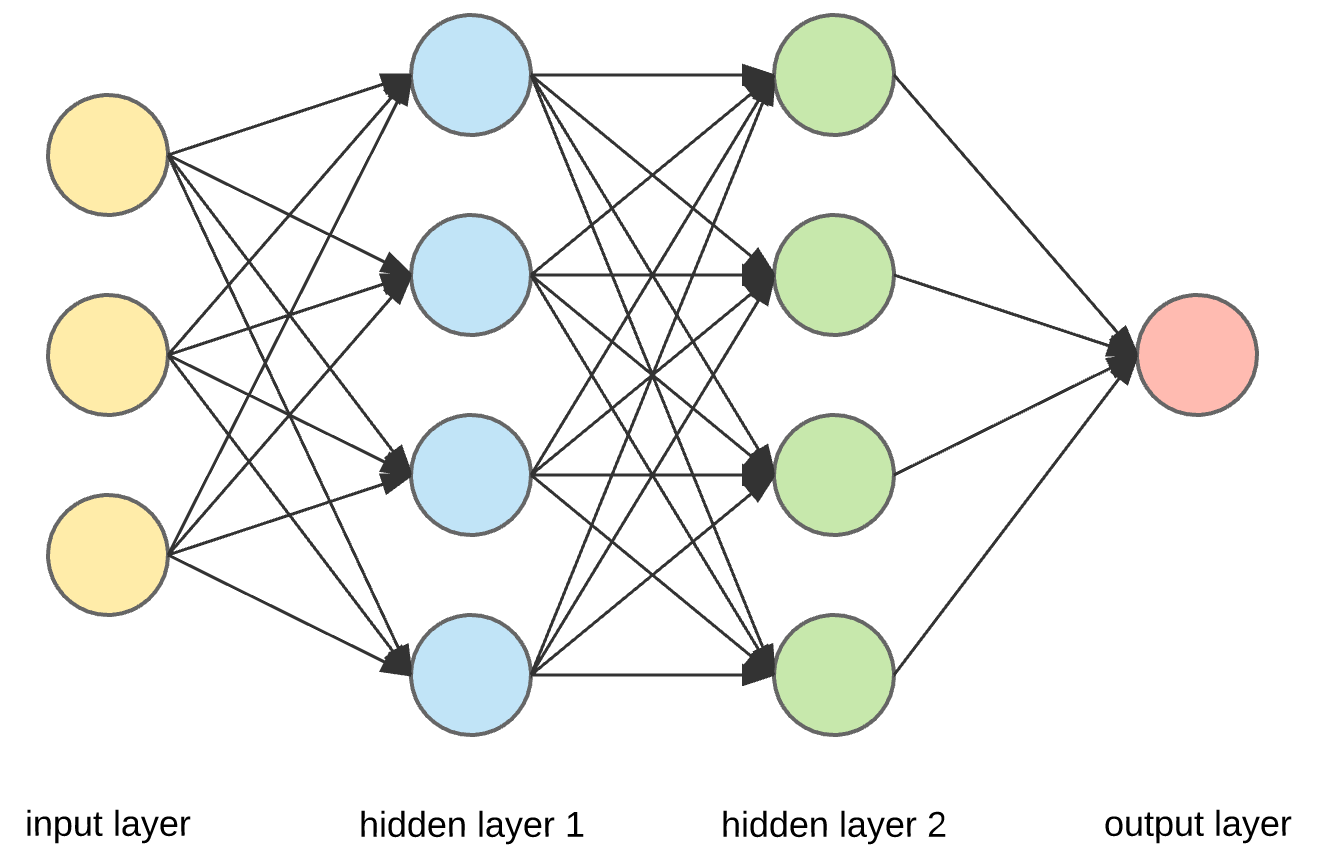
\includegraphics[width=0.49\textwidth]{network}
	%\caption{Feedforward Deep Neural Network. (Retrieved from https://towardsdatascience.com)}
	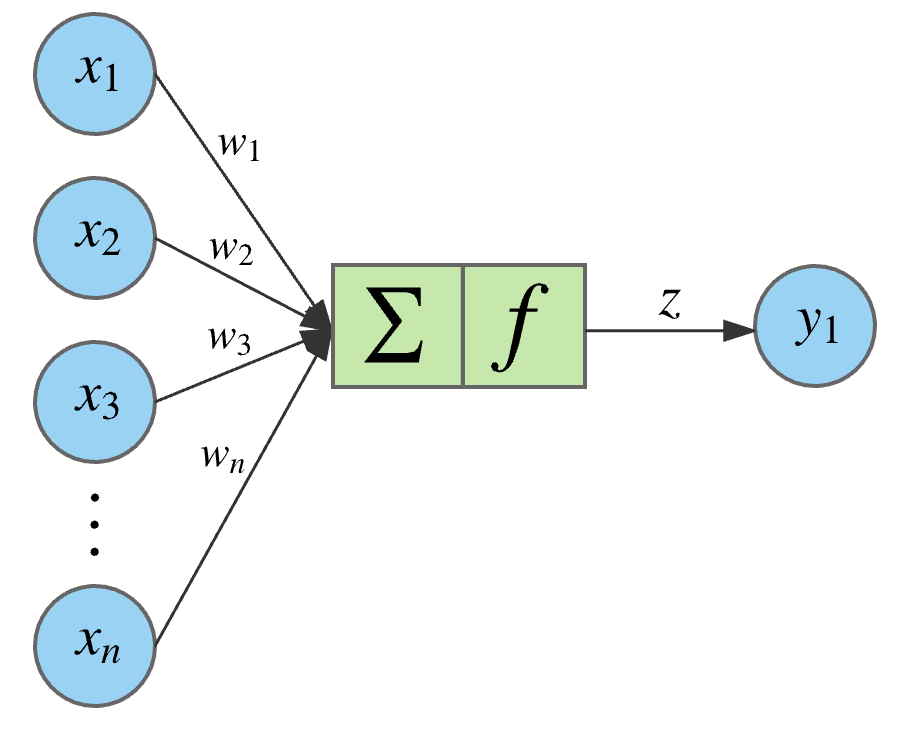
\includegraphics[width=0.49\textwidth]{neuron}
	\caption{Feedforward Deep Neural Network and Single Neuron - McCulloch-Pitts model. (Retrieved from https://towardsdatascience.com)}
	\label{neural}
	\end{figure}

\newpage

\section{Neural Network Training}
Training a neural network is an optimization problem as we will discuss in this section. Ruoyu Sun covers in \cite{sun2019optimization} the current theory and algorithms for optimizing deep neural networks, upon which much of this section is based.

In a supervised learning problem a dataset of inputs and desired outputs is given: $x_i \in \mathbb{R}^{d_x}, y_i \in \mathbb{R}^{d_y}, i = 1,\dots,n$ with $x_i$ the input vectors, $y_i$ the desired output vectors and $n$ the number of data points. We want the network to predict the output $y_i$ based on the information in $x_i$, i.e. we want the network to learn the underlying mapping that connects the data. A standard fully connected network can be expressed as a combination of function composition and matrix multiplication as follows:


\begin{equation}
         f_W(x) = W_L\sigma(W_{L-1}\sigma(...W_1\sigma(W_0x)...))
\end{equation}

where $L$ is the number of hidden layers in the network, $W_j$ are matrixes of dimension $d_j \times d_{j-1}, j=1 \dots L$ containing the connection weights and $\sigma$ is the activation function. The bias vectors $b_i$ have been omitted from this equation for clarity.

This function can also be defined recursively, which will be useful for later interpreting the network in an optimal control context.

\begin{equation}
	\begin{aligned}
	z_0 &= x \\
	z_{k+1} &= \sigma(W_kz_k + b_k), & k = 0,...,L-1 \\
	f_W(x) &= W_Lz_L + b_L \\
	\end{aligned}
\label{st-eq}
\end{equation}
where $b_k$ are the bias vectors, and the other variables are as defined before.

We want to pick the parameters of the neural network so that the predicted output $\hat{y}_i = f_W(x_i)$ is as close as possible to the true output $y_i$ for a certain distance metric $\mathit{l(\cdot,\cdot)}$. Thus the optimization problem can be written as follows:

\begin{equation}
\begin{aligned}
& \underset{W}{\text{minimize}}
& C(W) &= \sum\limits_{j=0}^{n}l(y_j,f_W(x_j)) \\
\end{aligned}
\label{op-eq}
\end{equation}

In this thesis only regression problems will be considered, where $l(x,y)$ is the quadratic loss function $l(x,y) = ||x^2-y^2||$, a.k.a. mean square error (MSE). For classification problems cross entropy loss is the most common cost function: $l(x,y) = x\log(y)+(1-x)\log(y)$. Writing down equation \ref{op-eq} using the MSE gives the following optimization problem:

\begin{equation}
\begin{aligned}
& \underset{W}{\text{minimize}}
& C(W) &= \sum\limits_{j=0}^{n}||y_j - f_W(x_j)||^2_2 \\
\end{aligned}
\label{op2-eq}
\end{equation}

Most methods for solving equation \ref{op-eq} are based on gradient descent (GD). This algorithm uses the gradient of the loss function to search for a local minimum:
\begin{equation}
W_{k+1} = W_{k} - \eta_k\nabla F(W_k)
\label{gd-eq}
\end{equation}

where $\eta_k$ is the step size (a.k.a. "learning rate") and $\nabla F(W_k)$ is the gradient of the loss function at the $k$-th iterate.

\section{Neural network training as an optimal control problem}
Neural network training can also be seen as an optimal control problem. A neural network is a multi-stage dynamical system, where every layer is a stage. The dynamics are ruled by the equations \ref{st-eq}. In optimal control the following objective cost function is considered:

\begin{equation}
E(\theta) = \sum\limits_{s=1}^{L-1}g^s(a^s,\theta^s) + h(a^L)
\end{equation}


$a^s$ and $\theta^s$ are the state and decision vectors at stage $s$, and $g^s$ and $h$ are the immediate cost at stage $s$ and the terminal cost, respectively. In neural network training the immediate costs are usually dropped. If the terminal cost is taken to be the MSE, the same cost function as in equation \ref{op2-eq} is found. The terminology and notation differences have been summarized in table \ref{trans-tbl}. Using neural network terminology the optimal control problem to be solved is the following:

\begin{equation}
	\begin{aligned}
	& \underset{W}{\text{minimize}}
	& & \sum\limits_{j=0}^{n}||W_Lz_{L,j} - y_j||^2_2 \\
	& \text{subject to}
	& & z_{0,j} = x_j \\
	& & & z_{k+1,j} = \sigma(W_kz_{k,j} + b_k,0), &k = 0,\ldots,L-1,j = 1,\ldots,n
	\end{aligned}
	\label{ocp-eq}
\end{equation}


\begin{table}
\centering
\begin{tabular}{c | c | c | c}
Notation & Optimal Control & Neural Network & Notation\\ \hline
$\theta$ & decision variables & weight parameters & $W$\\
$a$ & state variables & (neuron) activation & $z$\\
& stage & layer \\
\end{tabular}
\label{trans-tbl}
\end{table}


\section{Backpropagation}
The current standard algorithm for training a neural network is backpropagation (BP). It works by efficiently calculating the gradient for GD (equation \ref{gd-eq}). It was discovered and popularised in the context of neural networks by Rumelhart, Hinton \& Williams (1986) \cite{Rumelhart1986}. But it has been shown that by viewing the problem in an optimal control context, the backpropagation algorithm is the same as the gradient formulas discovered by Kelley and Bryson in 1960 \cite{dreyfus1990}.

This section will explain how backpropagation works, it will largely follow and summarize \cite{Nielsen2015}. Essentially BP evaluates the derivative of the cost function from the end to the front of the network, i.e. "backwards". It works on each input-output pair individually, with the full gradient given by the averaging over all pairs.

Given an input-output pair $(x,y)$, the loss is:
\begin{equation}
C(y,W_L\sigma(W_{L-1}...\sigma(W_1\sigma(W_0x))))
\end{equation}
The loss is calculated forwards by evaluating the network, starting with the input $x$. Note the weighted input at each layer as $\nu_l = W_{l-1}z_{l-1} + b_{l-1}$. The activations $z_l = \sigma(\nu_l)$ and the derivatives $f'_l = \sigma'(\nu_l)$ at each layer $l$ are stored for the backward pass.

The total derivative of the cost function $C$ evaluated at the value of the network on the input $x$ is given by the chain rule:
\begin{equation}
	\begin{aligned}
	\frac{dC}{dx} &= \frac{dC}{dz_L}\cdot \frac{dz_L}{d\nu_L}\cdot \frac{d\nu_L}{dz_{L-1}}\cdot \frac{dz_{L-1}}{d\nu_{L-1}} \cdot \frac{d\nu_{L-1}}{dz_{L-2}}\dots\frac{dz_0}{d\nu_0}\cdot\frac{d\nu_0}{dx} \\
	&= \frac{dC}{dz_L}\cdot 1 \cdot W_L \cdot f'_{L-1} \cdot W_{L-1} \dots f'_0 \cdot W_0 \\
	\end{aligned}
\end{equation}

The gradient $\nabla$ is the transpose of the derivative.

\begin{equation}
\nabla_xC = W_0^T \cdot f'_0 \dots W_{L-1}^T \cdot f'_{L-1} \cdot W_L^T \cdot \nabla_{z_L}C
\end{equation}

Backpropagation then essentially evaluates this expression from right to left. For this operation an auxiliary variable $\delta_l$ is introduced which is interpreted as the "error at layer l":

\begin{equation}
\delta_l = f'_l \cdot W_{l+1}^T \dots W_{L-1}^T \cdot f'_{L-1} \cdot W_L^T \cdot \nabla_{z_L}C
\end{equation}

The gradient of the weights in layer $l$ is then:

\begin{equation}
\nabla_{W_l}C=\delta_l(z_l)^T
\end{equation}

$\delta_l$ can easily be computed recursively:

\begin{equation}
\delta_{l-1}  = f'_{l-1} \cdot W_l^T \cdot \delta_l
\end{equation}

In this way the gradients of the weights are computed with only a few matrix operations per layer in a back to front fashion, this is backpropagation.


\section{Direct Multiple Shooting Method}
It has been shown that the BP algorithm detailed in the previous setting can be derived in an optimal control context in the spirit of dynamic programming \cite{mizutani2000}. But control theory has many other solution methods for OCPs. One of the more well known one is the direct multiple shooting method (DMS) \cite{bock1984multiple}.

In this method the state variables in the non-linear program (NLP), equation \ref{ocp-eq}, are not eliminated using the dynamics. Instead the dynamics are kept as constraints to the NLP. This leads to a much larger NLP, but it will be more structured. This is in contrast to the direct single shooting method, where the dynamics are eliminated, leading to a small, but highly non-linear problem. The BP algorithm is analogous to a direct single shooting method.

The total number of variables that will be optimized for in a neural network is quite large. For a fully connected neural network of width $W$, depth $L$, there will be $\mathcal{O}(W^2L)$ weights to be optimized, a.k.a. decision variables in control theory. This is true for both BP and DMS. But for DMS, another $\mathcal{O}(WLN)$ state variables are added, with $N$ the number of training samples. In control theory the tradeoff for making the problem larger in this way is that the problem becomes less non-linear. In practice this often makes the NLP easier to solve, or come to better solution and that is why DMS is a common choice. For neural networks this could let the algorithm get stuck in a "bad" local minimum less often.

\section{Goal of the Thesis}

The main goal of this thesis is to implement the direct shooting method for training neural networks, and compare it to the industry standard backpropagation algorithm. First an initial exploration of the method will be conducted in MATLAB, then the algorithm will be implemented in python using an Augmented Langrangian Method.

The code will be compared to common gradient descent and stochastic gradient descent algorithms used in practice such as ADAM \cite{kingma2017adam}. They will be compared in terms of speed, scalability and reliability for a number of test problems.

In particular the objective will be to see if this algorithm can better handle known challenges for current training algorithms, such as the "vanishing/exploding gradient problem", or convergence to "bad local minima" (Goodfellow et al. \cite{Goodfellow-et-al-2016}, Sec. 8.2).



